\documentclass{sintefbeamer}

% packages, font, color, and newcommands
\usepackage{amsfonts, amsmath, oldgerm, lmodern, bm}
% \usepackage[font={footnotesize}]{caption}
\usepackage{natbib}
\usepackage{url}
\usepackage{tikz}
\usepackage{amssymb}
\usepackage{amsmath}
\usepackage{amsthm}
\usepackage{mathrsfs}
\usepackage{empheq}
\usepackage{mdframed}
\usepackage{bm}
\usepackage{animate}
\usepackage{xcolor,colortbl}
\usepackage{graphicx}
\bibliographystyle{apalike}
\usefonttheme{serif}
\usetikzlibrary{calc}

\title{Theoretical prediction of the Reynolds stress in low inertial buoyant emulsion.}
\subtitle{Based on the nearest particle statistic}
\author{\href{http://basilisk.fr/sandbox/fintzin/Rising-Suspenion/RS.c}{\underline{N. Fintzi}\footnote{IFP \'Energies Nouvelles, France}$^{,2}$}, JL. Pierson$^1$ and S. Popinet\footnote{Sorbonne Universit\'e, France}}
% \date{Created on May 22, 2022}

\titlebackground{image/700drop.png}

% document body
\addtobeamertemplate{navigation symbols}{}{%
    \usebeamerfont{footline}%
    \usebeamercolor[fg]{footline}%
    % \hspace{1em}%
    % \vspace{1em}%
    \insertframenumber/\inserttotalframenumber
}
\usepackage{stmaryrd}

\usepackage{amsmath}


\begin{document}
\maketitle


\begin{frame}
  \frametitle{Problem statement}

  \begin{figure}[h!]
    \centering
    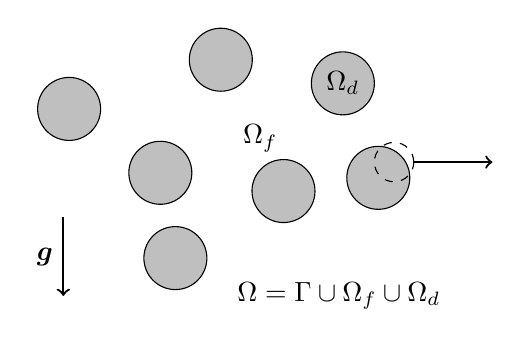
\begin{tikzpicture}
        \foreach \x/\y/\ra/\r/\th in 
        {1/3/0.4/0.4/0,
        2.55/2.7/0.4/0.4/0,
        0.5/0.4/0.4/0.4/10,
        2/1/0.4/0.4/10,
        3/1.5/0.4/0.4/0,
        0.5/1.5/0.4/0.4/10,
        -0.5/2.5/0.4/0.4/10}{
            \draw[fill=gray!50,rotate=\th](\x,\y) ellipse(\r cm and \ra cm);
        }
        \draw[dashed](3.2,1.7)circle(0.25);
        % \draw[thick,->](3.2,1.7)++(0.1767,0.1767)--++(0.4,0.4)--++(1,0);
        \draw[thick,->](3.2,1.7)++(0.25,0)--++(1,0);
        \draw[thick,->](-1,1)--++(0,-1)node[midway, left]{$\bm g$};
        \draw(2.55,2.7)node{$\Omega_d$};
        \draw(1.5,2)node{$\Omega_f$};
        \draw(2.5,0)node{$\Omega = \Gamma \cup \Omega_f \cup \Omega_d$};
        % \draw(2.5,-1)node{$\Gamma = \sum_\alpha \Gamma_\alpha$};
        % \draw(2.5,-0.5)node{$\Omega_d = \sum_\alpha \Omega_\alpha$};
    \end{tikzpicture}
    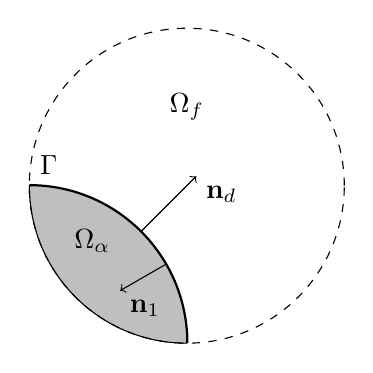
\begin{tikzpicture}
        \draw[very thick](0:2)arc(0:90:2)node[above right]{$\Gamma$};
        \draw[fill=gray!50](0:2)arc(0:90:2)arc(180:270:2);
        \draw[dashed](2,2)circle(2);
        \draw[->](1.42,1.42)--++(0.7,0.7)node[below right]{$\textbf{n}_d$};
        \draw[->](1.73,1)--++(-0.577,-0.333)node[below right]{$\textbf{n}_1$};
        \draw(2,3)node{$\Omega_f$};
        \draw(0.8,1.3)node{$\Omega_\alpha$};
    \end{tikzpicture}
    \caption{Domain definitions and scheme of the topology of dispersed two-phase flows.
    $\rho_k$ and $\mu_k$ is the density and viscosity of phase $k$, respectively. }
    \label{fig:Scheme}
\end{figure}

The phase and interface indicator functions : 
\begin{align*}
  \chi_k(\textbf{x},t) =  \left\{
    \begin{tabular}{cc}
      $1 \;\text{if} \;\textbf{x} \in \Omega_k(t)$\\
      $0 \;\text{if} \;\textbf{x} \notin \Omega_k(t)$
    \end{tabular}
    \right.
    % \text{for $k = 1,2$},
    % \label{eq:PIF}
    &&
  \delta_I(\textbf{x},t) =  \left\{
    \begin{tabular}{cc}
      $1 \;\text{if} \;\textbf{x} \in \Gamma(t)$\\
      $0 \;\text{if} \;\textbf{x} \notin \Gamma(t)$
    \end{tabular}
    \right.,
    \label{eq:PIF_I}
\end{align*}

\end{frame}



\begin{frame}
  \frametitle{Local scale mass and momentum laws.}
  The mass $\rho_k$ and momentum $\rho_k \textbf{u}_k^0$, conservation in the volumes follow :
\begin{align}
  \div  \textbf{u}_k^0
  &= 
  0
  \;\;\;\; 
  \text{in} 
  \;\;\;\; 
  \Omega_k(t)\\
  \pddt (\rho_k \textbf{u}_k^0)  
  + \div (
      \rho_k \textbf{u}_k^0\textbf{u}_k^0
      - \bm{\sigma}_k^0 
      )
  &= 
  \rho_k \textbf{g}
  \;\;\;\; 
  \text{in} 
  \;\;\;\; 
  \Omega_k(t)
\end{align}
And at the interfaces : 
\begin{align*}
  \Jump {\textbf{u}_k^0}
  = 0,\;\;\;
  \Jump {\bm{\sigma}_k^0}
  = 
   \gamma\textbf{n}(\div \textbf{n})
   \;\;\;\; 
   \text{at} 
   \;\;\;\; 
   \Gamma(t)
\end{align*}
\begin{definition}
  \begin{itemize}
    \item $\Jump{\ldots} = \sum_k \ldots$ Jump condition.  
    \item The superscript $^0$ indicated that it is a local quantity.
    \item $\rho_k$  density of phase $k$. 
    \item $\textbf{u}_k$  Velocity of phase $k$.
    % \item $\textbf{b}_k^0 = \rho_k \textbf{g}$  local body force.  
    \item $\gamma$ and $\div \textbf{n}$  surface tension coefficient and curvature of the surface.  
    \item $\bm\sigma_f^0 = -p_f^0 \textbf{I} + \mu_f (\grad \textbf{u}_f^0+^\dagger\grad \textbf{u}_f^0)$ Newtonian stress tensor of the fluid phase. 
    % \item $\bm\sigma_d^0 = \textbf{Udefined}$ Solid phase stress. 
  \end{itemize}
\end{definition}

\end{frame}


% \begin{frame}
%   \frametitle{Two-fluid formulation of the momentum equation.}
% %   Transport of the phase indicator function, 
% %   \begin{align}
% %     \pddt \chi_k
% %     + \textbf{u}_I^0 \cdot \grad \chi_k
% %     = 0,&&
% % % \end{align}
% % % \begin{align}
% %     \grad \chi_k
% %     = - \delta_I \textbf{n}_k
% %   \end{align}
%   Multiplying the momentum equation by $\chi_k$ gives two-fluid formulation of the momentum equation :
  
%   \begin{align}
%     \label{eq:mass}
%     \pddt (\chi_k\rho_k)  
%     + \div (
%         \chi_k\rho_k \textbf{u}_k^0
%         )
%     &= 0\\
%     \pddt (\chi_k\rho_k \textbf{u}_k^0)  
%     + \div (
%         \chi_k\rho_k \textbf{u}_k^0\textbf{u}_k^0
%         - \chi_k\bm{\sigma}_k^0 
%         )
%     &= 
%     \chi_k\textbf{b}_k^0
%     + \underbrace{\delta_I \bm{\sigma}_k^0\cdot\textbf{n}_k}_\text{Interphase momentum transfer}
%     \label{eq:momentim}
%   \end{align}

%   $\to$ notice that (\ref{eq:mass}) and (\ref{eq:momentim}) are defined over $\Omega$ thanks to $\chi_k$. 
%   Therefore, we are now able to apply the ensemble average procedure. 
% \end{frame}


\begin{frame}
  \frametitle{Ensemble average definition}
%   Let, $P(\FF)$ be the probability density function that describe the probability of finding the flow in the configuration $\FF$, were $\FF = (\lambda_1,\lambda_d,\lambda_3,\ldots)$ is a finite set of all the parameters describing the initial flow configuration.
% \footnote{Assuming that the flow can be described by a finite number of parameters related to both phase...}. 
% We define $d\mathscr{P} = P(\FF)d\FF$ as the probable number of flow in the incremental region of the particles' phase space $d\FF$ around $\FF$. 
% It follows from this definition, that the ensemble average of an arbitrary local property $f^0[\textbf{x},t;\FF]$ defined on the whole space $\Omega$, is,
The continuous and particle ensemble  averaged energy : 
\begin{align*}
  \phi_k (\textbf{x},t) = \avg{\chi_k }\\
  \phi_k \rho_k  \textbf{u}_k (\textbf{x},t) = \avg{\chi_k \rho_k \textbf{u}_k^0 }\\
  \phi_k \bm\sigma_k (\textbf{x},t) = \avg{\chi_k \bm\sigma_k^0 }\\
  % \phi_k \textbf{b}_k (\textbf{x},t) = \avg{\chi_k \textbf{b}_k^0 }
  \label{eq:1_avg}
\end{align*}
% \begin{equation}
%   n_p E_p(\textbf{x},t) = \avg{\sum_\alpha^N \delta(\textbf{x} - \textbf{x}_\alpha(\FF,t)) E_\alpha}
%   \label{eq:p_avg}
% \end{equation}
\begin{definition}
  \begin{itemize}
    \item $\avg{\ldots}$ ensemble average operator. 
    \item  $\phi_k (\textbf{x},t)$ volume fraction of the phase $k$. 
    \item Note that we dropped the superscript $^0$ on $\textbf{u}^0_k$ to indicate that $\textbf{u}_k$ is a macroscopic quantity. 
    % \item $n_p (\textbf{x},t) = \avg{\sum_\alpha^N \delta(\textbf{x} - \textbf{x}_\alpha(\FF,t))}$ number density of particles. 
    % \item  Both are linked through :   $\phi_d \rho_d= m_p n_p + \frac{1}{2}\grad^2 : (n_p\mathcal{M}_p)+\ldots$
  \end{itemize}
\end{definition}
\end{frame}

\begin{frame}
  \frametitle{Continuous phase averaged equations }
\begin{align*}
  \phi_d + \phi_f &= 1\\
  \pddt (\phi_f \rho_f)  
  + \div (\phi_f \rho_f\textbf{u}_f)
  &= 
  0\\
  \pddt (\phi_f \rho_f\textbf{u}_f)  
  + \div (
      \phi_f \rho_f\textbf{u}_f\textbf{u}_f
      + \bm{\sigma}_f^\text{eq}
  )
  &= 
  \phi_f  \rho_f \textbf{g}
  + 
  \underbrace{
    \avg{\delta_I \bm{\sigma}_f^0 \cdot \textbf{n}_f}
  }_\text{Interphase force}
\end{align*}
The \textbf{effective stress} is written :
$
  \bm{\sigma}_f^\text{eq}
  = 
   \underbrace{\rho_f\avg{\chi_f \textbf{u}_f'\textbf{u}_f'}}_\text{Reynolds stress}
    - \underbrace{\phi_f \bm{\sigma}_f}_\text{Newtonian stress},
$

\begin{enumerate}
  \item How to model $\rho_f\avg{\chi_f \textbf{u}_f'\textbf{u}_f'}$ in terms of the averaged fields unknown ?
  \begin{itemize}
    \item $\phi_d$ Droplets volume fraction 
    \item $\textbf{u}_p$ mean dispersed phase velocity
    \item $\textbf{u}_f$ mean fluid phase velocity
  \end{itemize}
\end{enumerate}

\end{frame}




\begin{frame}
  {In the case of buoyant suspension}

  Based on the analytical form of potential flow solution we propose :
  \begin{equation*}
    \avg{\chi_1 \textbf{u}_1'\textbf{u}_1'}
    = 
    \textbf{U}
    \textbf{U}
    k^{||}_1
    + 
    \left[
        \textbf{I} (\textbf{U}\cdot \textbf{U})
    -
    \textbf{U}
    \textbf{U}
    \right]
    k^{\bot}_1
\end{equation*}
\begin{itemize}
  \item $\textbf{U} = \textbf{u}_p - \textbf{u}_1$ interphase velocity. 
\end{itemize}
$\to$ where $k_{||}$ and $k^\bot$ are to coefficient to be determined by the use of DNS. 
\end{frame}

\begin{frame}
  \frametitle{Direct Numerical Simulation of buoyant emulsions}
  \begin{columns}
    \column{0.6\textwidth}
  \underline{Dimensionless parameters :} 
  \begin{itemize}
    \item \textit{Galileo} number : $Ga =\frac{\sqrt{\rho \Delta\rho gD^3}}{\mu} \in [5, 100]$
    \item \textit{Bond} number : $Bo = \frac{\Delta \rho g D^2}{\sigma} = 1$ 
    \item volume fraction of dispersed phase : $\phi = [0.01;0.2]$. 
    \item Density and viscosity ratio, $\rho_r=1.11$ and $\lambda= 10,1$. 
  \end{itemize}
  
  \begin{figure}
    \caption{Snapshot of a simulation at $T_g = 300$ for $\phi = 0.01$, $Ga = 75$ $\mu_r = 0.1$ and $N_b = 125$. In white : the interfaces, The background color map correspond to the pressure field. The grid represents the different core ($\le 729$ !).
    }
  \end{figure}
  \column{0.5\textwidth}
  \centering
  \href{file:///work/fintzin/BUBLLES_PROJECT/movies/layers.mp4}{\beamergotobutton{Play}}
  \includegraphics[width =  1.1\textwidth]{image/PHI_01_Ga_75.png}
  \end{columns}
\end{frame}

\begin{frame}
  \frametitle{Numerical results}

  \begin{figure}[h!]
    \centering
    \includegraphics[height=0.3\textwidth]{image/HOMOGENEOUS/fCA/Tf_l_1.pdf}
    % \includegraphics[height=0.3\textwidth]{image/HOMOGENEOUS/fCA/Bf_l_1.pdf}
    \includegraphics[height=0.3\textwidth]{image/HOMOGENEOUS/fCA/Tf_l_10.pdf}
    % \includegraphics[height=0.3\textwidth]{image/HOMOGENEOUS/fCA/Bf_l_10.pdf}
    \caption{(left) Dimensionless turbulent kinetic energy in terms of the \textit{Galileo} number for different $\phi$. (dots) Numerical simulations.
    The symbols correspond to different volume fraction ($\bullet$) $\phi = 1\%$, ($\blacktriangle$) $\phi = 5\%$, ($\blacksquare$) $\phi = 10\%$, ($\blacklozenge$) $\phi = 15\%$ and ($\blacktriangleright$) $\phi = 20\%$.}
    \label{fig:Tf_Bf}

    \begin{itemize}
      \item $\lambda = 1,10 = \mu_d/\mu_f$ is the viscosity ratio. 
    \end{itemize}
\end{figure}

\end{frame}
\begin{frame}
  {What about the particle velocity variance }

  \begin{equation*}
    \pavg{\textbf{u}_\alpha'\textbf{u}_\alpha'}
    = f(\avg{\chi_1 \textbf{u}_1'\textbf{u}_1'})
\end{equation*}

\vfill

$\to$ How to link $ \avg{\chi_1 \textbf{u}_1'\textbf{u}_1'}$ and $\pavg{\textbf{u}_\alpha' \textbf{u}_\alpha'}$ ?
\end{frame}

\begin{frame}
  \frametitle{Particle Kinetic energy equations }
  \footnotesize
  \begin{align*}
    &\pddt \left(n_p m_p k_p\right)
    + \div \left(n_p
    m_p k_p \textbf{u}_p 
    + \textbf{q}^k_p
    % + \textbf{u}_p \cdot \bm{\sigma}_p^\text{eq}
    \right)
    = 
    - \bm{\sigma}_p^\text{eq}  :\grad \textbf{u}_p
    + \pavg{\textbf{u}_\alpha'\cdot\intS{\bm{\sigma}_\text{ext}^0 \cdot \textbf{n}}}\\
    &\pddt \left(n_p W_p\right)
    + \div 
    (n_p W_p
    \textbf{u}_p 
    +  \textbf{q}_p^\text{w}
    )
    = 
    - \pOavg{{\bm{\sigma}_2^0 : \grad\textbf{u}_2^0}}
    + \pSavg{{\textbf{w}_2^0 \cdot \bm{\sigma}_\text{ext}^0 \cdot  \textbf{n}}}
    - \pavg{\ddt{ s_\alpha}}
\end{align*}
where we have defined, 
\begin{align*}
    \textbf{q}_p^\text{k}
    = m_p \pavg{\textbf{u}_\alpha' k_\alpha} \\
    \textbf{q}_p^\text{W}
    = m_p \pavg{\textbf{u}_\alpha' W_\alpha} 
\end{align*}

\begin{itemize}
  \item $\textbf{w}_2^0 = \textbf{u}_2^0 - \textbf{u}_\alpha$ is the local velocity relative to the particle center of mass. 
  \item $W_p = \intO{\rho_2\textbf{w}_2^0\cdot \textbf{w}_2^0}$
  Is the mean internal kinetic energy of the particles (such as rotation and fluid internal motion...)
  \item $\pavg{\ddt{ s_\alpha}}$ mean time derivative of the particle surface energy. 
  \item $\pOavg{{\bm{\sigma}_2^0 : \grad\textbf{u}_2^0}}$ energy dissipation due to internal stresses. 
\end{itemize}

$\to$ \underline{Is there a direct impact of  energy dissipation due to collision in the equation  of  $k_p$ ?
}

$\to$ \underline{What is the meaning of $\pavg{\textbf{u}_\alpha'\cdot\intS{\bm{\sigma}_\text{ext}^0 \cdot \textbf{n}}}$ when it comes to contact forces  ?}
\end{frame}

\begin{frame}
  {Fluid kinetic energy equation :}
  \small
  \begin{multline*}
    \pddt (\phi_1\rho_1k_1)  
    + \div (
      \phi_1\rho_1k_1\textbf{u}_1
      + \textbf{q}_1^\text{k} 
      )
      = 
      - \avg{\chi_1\bm{\sigma}_\text{ext}^0 : \grad \textbf{u}_1^0}
      - \bm{\sigma}_f^\text{eq} : \grad \textbf{u}_1\\
      + (\textbf{u}_1 - \textbf{u}_p)
      \cdot \pSavg{{\bm{\sigma}_\text{ext}^0 \cdot \textbf{n}}}
      - \pavg{ \textbf{u}_\alpha' \cdot \intS{  \bm{\sigma}_\text{ext}^0 \cdot \textbf{n}}}
      - \pavg{ \intS{\textbf{w}_2^0 \cdot \bm{\sigma}_\text{ext}^0 \cdot \textbf{n}}} 
  \end{multline*}
  with, 
  \begin{multline*}
    \textbf{q}_1^\text{k}
      = \rho_1 \avg{\chi_1 \textbf{u}_1' k_1} 
      - \avg{\chi_1 \textbf{u}_1' \cdot \bm{\sigma}_\text{ext}^0}
      + (\textbf{u}_1 - \textbf{u}_p)\cdot
      \pSavg{{\textbf{r}\bm{\sigma}_\text{ext}^0 \cdot \textbf{n}}}\\
      + \pavg{ \textbf{u}_\alpha' \cdot \intS{ \textbf{r} \bm{\sigma}_\text{ext}^0 \cdot \textbf{n}}}
      + \pavg{ \intS{\textbf{r}\textbf{w}_2^0 \cdot \bm{\sigma}_\text{ext}^0 \cdot \textbf{n}}}
  \end{multline*}
\end{frame}


\begin{frame}
  \frametitle{Internal energies equations}
\begin{align*}
  \pddt (\phi_f\rho_fe_f)  
  + \div (
      \phi_f \rho_fe_f\textbf{u}_f
      +
      \textbf{q}_f^\text{e} 
      )
  = 
  \avg{\chi_f\bm{\sigma}_f^0 : \grad \textbf{u}_f^0}
  + \pSavg{{\textbf{q}_f^0 \cdot \textbf{n}}} \\
  \pddt \left(n_p m_p e_p\right)
  + \div \left(n_p
  m_p e_p \textbf{u}_p 
  +  \textbf{q}_p^\text{e}
  \right)
  = 
  + \pOavg{{\bm{\sigma}_2^0 : \grad\textbf{u}_2^0}}
  - \pSavg{{\textbf{q}_f^0\cdot \textbf{n}}}
\end{align*}
  
\begin{itemize}
  \item $e_p$ and $e_f$ mean internal energy of the particle  and fluid phase. 
  \item $\textbf{q}_f^0\cdot \textbf{n}$ Local heat fluxes.
  \item $\bm{\sigma}_f^0 : \grad \textbf{u}_f^0$ and $\bm{\sigma}_2^0 : \grad \textbf{u}_2^0$ : Dissipation in the fluid and particle phase. 
\end{itemize}
\end{frame}

\begin{frame}{Energy transfer accors phases and scales}
  \begin{center}
    \tikzstyle{quadri}=[rectangle,draw]
    \begin{tikzpicture}
        \node[quadri] (u2) at (0,0){$(u_p)^2 / 2$};
        \node[quadri] (kp) at (4,0){$(k_p)$};
        \node[quadri] (Wp) at (8,0){$(W_p)$};
        \node[quadri] (ep) at (12,0){$(e_p)$};
        \node[quadri] (u12) at (2,-3){$\frac{\rho_f}{2}(u_f)^2$};
        \node[quadri] (k1) at (6,-3){$k_f$};
        \node[quadri] (e1) at (10,-3){$e_f$};
        \draw[->] (u2)--(kp)node[midway,above]{\footnotesize $\bm{\sigma}^\text{eq}:\grad \textbf{u}_f$};
        \draw[<->] (u2)--(u12) node[midway,left]{\footnotesize $\textbf{f}_{p} $};
        % \draw[<->,text width=2cm] (kp)--(u12) node[midway,left]{\footnotesize $+  n_p v_p \textbf{u}_p \cdot 
        % (\rho_2 \textbf{g} - \grad p_f)
        % + n_p \textbf{u}_p \cdot \textbf{f}_{pm} - \textbf{F}_\text{pfp}$};
        \draw[<->] (k1)--(u12) node[midway,below]{\footnotesize $\bm{\sigma}^\text{eq}_f:\grad \textbf{u}_f$, $\textbf{f}_p$};
        \draw[<->] (k1)--(e1) node[midway,below]{\footnotesize $\avg{\chi_f \bm{\sigma}_f^0 : \grad\textbf{u}_f^0}$};
        \draw[<->,sloped] (k1)--(kp) node[midway,below]{\footnotesize $\pavg{\textbf{f}_\alpha \cdot \textbf{u}_\alpha'}$};
        \draw[<->] (k1)--(u2) node[midway,below]{\footnotesize $\textbf{f}_p$};
        \draw[<->,sloped] (k1)--(Wp) node[midway,below]{\footnotesize $\intS{{\textbf{w}_2^0\cdot \bm{\sigma}_\text{ext}\cdot \textbf{n}}}$};
        % \draw[->] (kp)--(Wp)node[midway,above]{$(\textbf{u}_\alpha' \cdot \textbf{f}_\alpha')_p$};
        \draw[->] (Wp)--(ep)node[midway,above]{\footnotesize $\pOavg{\bm{\sigma}_2^0 : \grad \textbf{u}_2^0}$};
        \draw[->] (e1)--(ep)node[midway,above,sloped]{\footnotesize $\pSavg{\textbf{q}_f^0 \cdot \textbf{n}}$};
    \end{tikzpicture}
\end{center}
\begin{itemize}
  \item $\textbf{f}_p =  \pSavg{\bm{\sigma}_\text{ext} \cdot \textbf{n}}$ Interphase force. 
  \item $u_p^2$, and $u_f^2$ are the macroscopic kinetic energies
  \item $k_p$, and $k_f$ are the fluctuating kinetic energies.
  \item $W_p$ is the particles internal kinetic energy.
  \item $e_p$ and $e_f$ are the internal energies.
\end{itemize}
\end{frame}

\begin{frame}
  \frametitle{The ensemble average fluid phase Reynolds stress}
  \begin{equation*}
    \avg{\chi_k \textbf{u}'_k\textbf{u}'_k}(\textbf{x},t)
    % = \int \nstavg{\chi_k \textbf{u}_k^0\textbf{u}_k^0}  P_{nst}(\textbf{x},t,\textbf{r}) d\textbf{r}
    % - \phi_k \textbf{u}_k\textbf{u}_k
    = \int  \chi_k \textbf{u}^0_k\textbf{u}^0_k(\textbf{x},t,\CC) P(\CC)d\CC 
    - \phi_k \textbf{u}_k\textbf{u}_k
\end{equation*}

\begin{itemize}
  \item $\textbf{u}_k^0$ local instantaneous velocity fields;
  \item $\chi_k$ phase indicator function;
  \item $\textbf{u}_k$ phase averaged velocity fields;
  \item $\phi_k$ volume fraction;
  \item $\CC$ a configuration of the flow;
  \item $P(\CC)$ probability density of $\CC$.
\end{itemize}


\underline{How to find a theoretical expression ??? }
\end{frame}
\begin{frame}
  \frametitle{L.Van Wijngaarden approach for potential flow.}

The potential flow solution of an isolated translating spheres is :
\begin{equation*}
  \textbf{u}'_\text{potential}
  = \frac{a^3 \textbf{U}}{2}\left(\frac{1}{r^3} - \frac{3 \textbf{xx}}{r^5}\right).
  \text{    for    }r>a
\end{equation*}

Therefore, the Reynolds stress approximation in homogeneous dilute suspension of spherical bubbles can be written Wijngaarden(1976): 
  \begin{align*}
    \avg{\chi_k \textbf{u}'_k\textbf{u}'_k}(\textbf{x},t)
    &\approx \int \textbf{u}'_\text{potential}\textbf{u}'_\text{potential}  P_1(\textbf{x},t,\textbf{r}) d\textbf{r}
    - \phi_k \textbf{u}_k\textbf{u}_k\\
    &= \phi_k \left(\frac{3}{20} U^2\textbf{I} + \frac{1}{20}\textbf{UU} \right)
    % = \int  \chi_k \textbf{u}^0_k\textbf{u}^0_k(\textbf{x},t,\CC) P(\CC)d\CC 
    % - \phi_k \textbf{u}_k\textbf{u}_k
\end{align*}


\begin{itemize}
  \item $P_1(\textbf{r}) = n_p$ is the probability of finding a particle center of mass at \textbf{r} which is equal to the number density $n_p$. 
  \item \textbf{U} is the drift velocity between phases. 
  \item $a$ is the radius of the spheres. 
  % \item This relation is valid for infinitely dilute suspension $n_p \to \infty$
  \item The integral converge because $\textbf{u}_\text{potential}  \sim r^{-3}$
\end{itemize}

\end{frame}

\begin{frame}
  \frametitle{Stokes flow around a translating spherical drop}
  The stokes flow solution of an isolated translating drop is :

  \begin{equation*}
    \textbf{u}_\text{stokes} 
    = \left(\frac{ \textbf{I}}{r} + \frac{\textbf{rr}}{r^3}\right)  \frac{1}{4}\left(\frac{3\lambda + 2}{\lambda +1}\right) a \textbf{U}
    - \left(-\frac{\textbf{I}}{r^3} + \frac{3 \textbf{rr} }{r^5}\right)  \frac{1}{4}\left(\frac{\lambda}{\lambda +1}\right) a^3 \textbf{U}
  \end{equation*}

  \begin{itemize}
    \item $\lambda$ is the viscosity ratio.
  \end{itemize}
  
  Let's apply Wijngaarden approach on this solution : 
  \begin{align*}
    \avg{\chi_k \textbf{u}'_k\textbf{u}'_k}(\textbf{x},t)
    &\approx \int_a^\infty \textbf{u}'_\text{stokes}\textbf{u}'_\text{stokes}  P_1(\textbf{x},t,\textbf{r}) d\textbf{r}
    - \phi_k \textbf{u}_k\textbf{u}_k
    =\infty 
  \end{align*}
  \underline{The integral diverges since $\textbf{u}_\text{stokes} \sim r^{-1}$.}

  $\to$ Indeed in an infinitely dilute situation in stokes regime the Reynolds stress is indeed infinite.

  $\to$ Consequently, we must use another method which consider a finite volume fraction $\phi$. 
\end{frame}

\begin{frame}
  \frametitle{The nearest particle statistics decomposition}
  \begin{multline*}
    \avg{\chi_k \textbf{u}'_k\textbf{u}'_k}(\textbf{x},t)
    = 
    \underbrace{\int (\nstavg{\chi_k \textbf{u}^0_k}  \nstavg{\chi_k \textbf{u}^0_k} / (\nstavg{\chi_k})  P_{nst}(\textbf{x},t,\textbf{r}) d\textbf{r} }_\text{PWFs}
    \\+\underbrace{\int \nstavg{\chi_k \textbf{v}_k^0\textbf{v}_k^0}  P_{nst}(\textbf{x},t,\textbf{r}) d\textbf{r}}_\text{WIA}
    - \phi_k \textbf{u}_k\textbf{u}_k
  \end{multline*}

\begin{itemize}
  \item $\textbf{v}_k^0  = \textbf{u}_k^0 - \nstavg{\chi_k \textbf{u}^0_k} / \nstavg{\chi_k}$ is the fluctuation of the local velocity relative to the nearest averaged value. 
  \item This relation is exact and require no assumption. 
\end{itemize}
\end{frame}

\begin{frame}
  \frametitle{Potential flow solution with this method}
  \begin{multline*}
    \avg{\chi_k \textbf{u}'_k\textbf{u}'_k}(\textbf{x},t)
    = 
    {\int \textbf{u}_\text{potential} \textbf{u}_\text{potential}  P_{nst}(\textbf{x},t,\textbf{r}) d\textbf{r} }
    - \phi_k \textbf{u}_k\textbf{u}_k\\
    = \phi_k \left(\frac{3}{20} U^2\textbf{I} + \frac{1}{20}\textbf{UU} \right)
    \Gamma_\text{inc}(-1,\phi)\phi^2 e^\phi
  \end{multline*}

  \begin{itemize}
    \item \textbf{Hypothesis 1} : We considered $\textbf{v}^0_k =0$ since all the wake are considered similar. 
    \item \textbf{Hypothesis 2} : We considered $\textbf{u}_\text{nst} = \textbf{u}_\text{potential}$ since all the wake are considered similar. 
    \item We consider $P_{nst}(\textbf{x},t,\textbf{r}) = n_p e^{-4\pi n_p(r^3-a)/3}$ which is true for homogeneous flows. 
    \item $\Gamma_\text{inc}(a,x) = \int_x^\infty t^{a-1} e^{-t} dt $ is the incomplete gamma  function. 
  \end{itemize}

  $\to$ Notice that $\Gamma_\text{inc}(-1,\phi)\phi^2 e^\phi \rightarrow 1$ when $\phi \rightarrow 0$. Therefore, we recover  Wijngaarden(1976) solution in dilute regime. 
\end{frame}

\begin{frame}
  \frametitle{Reconstruction of the velocity fields from DNS}
  \begin{figure}[h!]
    \centering
    \begin{tikzpicture}
        \node (img) at (0,0)  {\includegraphics[height=0.25\textwidth]{image/HOMOGENEOUS/Stream/Stream_PHI_5_Ga_10_l_1.pdf}};
        \node (img) at (0.25\textwidth,0)  {\includegraphics[height=0.25\textwidth]{image/HOMOGENEOUS/Stream/Stream_PHI_5_Ga_100_l_1.pdf}};
        \node (img) at (0.5\textwidth,0)  {\includegraphics[height=0.25\textwidth]{image/HOMOGENEOUS/Stream/Stream_PHI_5_Ga_10_l_10.pdf}};
        \node (img) at (0.75\textwidth,0)  {\includegraphics[height=0.25\textwidth]{image/HOMOGENEOUS/Stream/Stream_PHI_5_Ga_100_l_10.pdf}};
    \end{tikzpicture}
    \caption{Nearest particle averaged velocity $\nstavg{\textbf{u}}(\textbf{r})$ for  $\phi = 5\%$ and $20\%$.
    Green lines : contour plots of the nearest averaged indicator function $\nstavg{\chi_d}(\textbf{r})$ (it represent the mean shape of the particles)}
    \label{fig:Stream}
  \end{figure}
  
  \begin{itemize}
    \item Close from the drop ($r=\mathcal{O}(a)$) we can see that $\textbf{u}_\text{nst} \approx \textbf{u}_\text{stokes}$. 
  \end{itemize}
\end{frame}

\begin{frame}
  \frametitle{Nearest particle statistic solution for translating drops in stokes flow :}
  \begin{multline}
    \avg{\chi_k \textbf{u}'_k\textbf{u}'_k}(\textbf{x},t)
    = 
    {\int_a^\infty \textbf{u}_\text{stokes} \textbf{u}_\text{stokes}  P_{nst}(\textbf{x},t,\textbf{r}) d\textbf{r} }
    - \phi_k \textbf{u}_k\textbf{u}_k
    \\=
-\left({{-\left(9\,\Gamma\left(-1 , \,\phi\right)\,\lambda^2\,\phi
^{{{4}\over{3}}}\,e^{\phi}\right)+\ldots}\over{\left(120\,\lambda^2+240\,\lambda+
120\right)\,\phi^{{{1}\over{3}}}}}\right)
\textbf{e}_U\textbf{e}_U + \ldots
\end{multline}
\begin{itemize}
  \item $\textbf{e}_U$ is the units vector in the direction of the drift velocity. 
\end{itemize}

\end{frame}

\begin{frame}
  \frametitle{Comparison with DNS results and experiments}
  \begin{figure}[h!]
    \centering    
    % \includegraphics[height = 0.25\textwidth]{image/upupexp.png}
    \includegraphics[height = 0.25\textwidth]{image/HOMOGENEOUS/fCA/cartellier.pdf}
    \includegraphics[height = 0.25\textwidth]{image/HOMOGENEOUS/fCA/Pseudo_turbe.pdf}
    \caption{
       Dimensionless \textbf{fluid phase pseudo kinetic energy} :
       (left) Comparison with the rising bubbles experiment of Cartellier (2009) with $Re \approx 10$. 
       (right) comparison with DNS for two viscosity ratio $\lambda =1,10$ and $Re \approx 1$ DNS. 
    }
    \label{fig:Cp}
\end{figure}  
\begin{itemize}
  \item The tendency in terms of $\phi$ and $\lambda$ are right.  
  \item Quantitative agreement at $\phi \ll 1$ and not at $\phi <1$ because of the interactions.  
  \item The present theory solution indeed diverge in $\phi \to 0$ 
\end{itemize}
\end{frame}

\begin{frame}
  \frametitle{Comparison with DNS results }
  \begin{figure}[h!]
    \centering    
    \includegraphics[height = 0.25\textwidth]{image/HOMOGENEOUS/fCA/Pseudo_turbe_coef.pdf}
    \caption{
       Coefficient of the Reynolds stress tensor in terms of the volume fraction $\phi$ for two viscosity ratio $\lambda =1,10$ and $Re \approx 1$ DNS. 
    }
    \label{fig:Cp}
\end{figure}  
Where we have defined :
\begin{equation*}
  \avg{\chi_1\textbf{u}_1'\textbf{u}_1'}
  = k^*_1 \left[
      \textbf{U}
      \textbf{U}
      (C_1  - C_2 )
      + \textbf{I} 
      (\textbf{U}\cdot\textbf{U})  (C_1+2/3) 
  \right]
\end{equation*}
\end{frame}


\begin{frame}
  \frametitle{Particle phase kinetic energy}
  Assuming \textbf{force free} particle in stokes flow one can also derive the Reynolds stress from nearest particle statistic. 
  \begin{figure}[h!]
    \centering    
    \includegraphics[height = 0.25\textwidth]{image/HOMOGENEOUS/fCA/Pseudo_turbeP.pdf}
    \caption{
       Dimensionless \textbf{granular temperature} in terms of the volume fraction $\phi$ for two viscosity ratio $\lambda =1,10$ and $Re \approx 1$ DNS. 
    }
    \label{fig:Cp}
\end{figure}  
\begin{itemize}
  \item The tendency in terms of $\phi$ and $\lambda$ are right.  
  \item Quantitative agreement at $\phi \ll 1$.  
\end{itemize}


\end{frame}
\begin{frame}
  {Perspectives}
  \begin{itemize}
    \item Takes in account interactions between particle with reflexion method 
    \item Takes in account inertial effect Using Ossen wake. 
    \item Can also compute : $\avg{\chi_1 \bm{\sigma}_1^0 : \grad  \textbf{u}_0^1}$ and other closure terms. 
  \end{itemize}
\end{frame}
\end{document}
